% Template for PLoS
% Version 3.1 February 2015
%
% To compile to pdf, run:
% latex plos.template
% bibtex plos.template
% latex plos.template
% latex plos.template
% dvipdf plos.template
%
% % % % % % % % % % % % % % % % % % % % % %
%
% -- IMPORTANT NOTE
%
% This template contains comments intended 
% to minimize problems and delays during our production 
% process. Please follow the template instructions
% whenever possible.
%
% % % % % % % % % % % % % % % % % % % % % % % 
%
% Once your paper is accepted for publication, 
% PLEASE REMOVE ALL TRACKED CHANGES in this file and leave only
% the final text of your manuscript.
%
% There are no restrictions on package use within the LaTeX files except that 
% no packages listed in the template may be deleted.
%
% Please do not include colors or graphics in the text.
%
% Please do not create a heading level below \subsection. For 3rd level headings, use \paragraph{}.
%
% % % % % % % % % % % % % % % % % % % % % % %
%
% -- FIGURES AND TABLES
%
% Please include tables/figure captions directly after the paragraph where they are first cited in the text.
%
% DO NOT INCLUDE GRAPHICS IN YOUR MANUSCRIPT
% - Figures should be uploaded separately from your manuscript file. 
% - Figures generated using LaTeX should be extracted and removed from the PDF before submission. 
% - Figures containing multiple panels/subfigures must be combined into one image file before submission.
% For figure citations, please use "Fig." instead of "Figure".
% See http://www.plosone.org/static/figureGuidelines for PLOS figure guidelines.
%
% Tables should be cell-based and may not contain:
% - tabs/spacing/line breaks within cells to alter layout or alignment
% - vertically-merged cells (no tabular environments within tabular environments, do not use \multirow)
% - colors, shading, or graphic objects
% See http://www.plosone.org/static/figureGuidelines#tables for table guidelines.
%
% For tables that exceed the width of the text column, use the adjustwidth environment as illustrated in the example table in text below.
%
% % % % % % % % % % % % % % % % % % % % % % % %
%
% -- EQUATIONS, MATH SYMBOLS, SUBSCRIPTS, AND SUPERSCRIPTS
%
% IMPORTANT
% Below are a few tips to help format your equations and other special characters according to our specifications. For more tips to help reduce the possibility of formatting errors during conversion, please see our LaTeX guidelines at http://www.plosone.org/static/latexGuidelines
%
% Please be sure to include all portions of an equation in the math environment.
%
% Do not include text that is not math in the math environment. For example, CO2 will be CO\textsubscript{2}.
%
% Please add line breaks to long display equations when possible in order to fit size of the column. 
%
% For inline equations, please do not include punctuation (commas, etc) within the math environment unless this is part of the equation.
%
% % % % % % % % % % % % % % % % % % % % % % % % 
%
% Please contact latex@plos.org with any questions.
%
% % % % % % % % % % % % % % % % % % % % % % % %

\documentclass[10pt,letterpaper]{article}
\usepackage[top=0.85in,left=2.75in,footskip=0.75in]{geometry}

% Use adjustwidth environment to exceed column width (see example table in text)
\usepackage{changepage}

% Use Unicode characters when possible
\usepackage[utf8]{inputenc}

% textcomp package and marvosym package for additional characters
\usepackage{textcomp,marvosym}

% fixltx2e package for \textsubscript
\usepackage{fixltx2e}

% amsmath and amssymb packages, useful for mathematical formulas and symbols
\usepackage{amsmath,amssymb}

% cite package, to clean up citations in the main text. Do not remove.
\usepackage{cite}

% Use nameref to cite supporting information files (see Supporting Information section for more info)
\usepackage{nameref,hyperref}

% line numbers
\usepackage[right]{lineno}

% ligatures disabled
\usepackage{microtype}
\DisableLigatures[f]{encoding = *, family = * }

% rotating package for sideways tables
\usepackage{rotating}

% Remove comment for double spacing
%\usepackage{setspace} 
%\doublespacing

% Text layout
\raggedright
\setlength{\parindent}{0.5cm}
\textwidth 5.25in 
\textheight 8.75in

% Bold the 'Figure #' in the caption and separate it from the title/caption with a period
% Captions will be left justified
\usepackage[aboveskip=1pt,labelfont=bf,labelsep=period,justification=raggedright,singlelinecheck=off]{caption}

% Use the PLoS provided BiBTeX style
\bibliographystyle{plos2015}

% Remove brackets from numbering in List of References
\makeatletter
\renewcommand{\@biblabel}[1]{\quad#1.}
\makeatother

% Leave date blank
\date{}

% Header and Footer with logo
\usepackage{lastpage,fancyhdr,graphicx}
\usepackage{epstopdf}
\pagestyle{myheadings}
\pagestyle{fancy}
\fancyhf{}
\lhead{
\includegraphics[width=2.0in]{PLOS-submission}}
\rfoot{\thepage/\pageref{LastPage}}
\renewcommand{\footrule}{\hrule height 2pt \vspace{2mm}}
\fancyheadoffset[L]{2.25in}
\fancyfootoffset[L]{2.25in}
\lfoot{\sf PLOS}

%% Include all macros below

\newcommand{\lorem}{{\bf LOREM}}
\newcommand{\ipsum}{{\bf IPSUM}}

%% END MACROS SECTION


\begin{document}
\vspace*{0.35in}

% Title must be 250 characters or less.
% Please capitalize all terms in the title except conjunctions, prepositions, and articles.
\begin{flushleft}
{\Large
\textbf\newline{Cursed Forest - A random forest implementation for `big' and `wide' data}
}
\newline
% Insert author names, affiliations and corresponding author email (do not include titles, positions, or degrees).
\\
Aidan O'Brien\textsuperscript{1},
Piotr Szul\textsuperscript{2},
Stephanie Li\textsuperscript{3},
James Doecke\textsuperscript{3},
Nick Ellis\textsuperscript{4},
Robert Dunne\textsuperscript{5}, and
Denis C. Bauer\textsuperscript{1,*}
%, with the Lorem Ipsum Consortium\textsuperscript{\textpilcrow}
\\
\bigskip
\bf{1} Health \& Biosecurity, CSIRO, Sydney, NSW, Australia
\\
\bf{2} Data61, CSIRO, Brisbane, QLD, Australia
\\
\bf{3} Health \& Biosecurity, CSIRO, Brisbane, QLD, Australia
\\
\bf{4} Oceans \& Atmosphere, CSIRO, Brisbane, QLD, Australia
\\
\bf{5} Data61, CSIRO, Sydney, NSW, Australia
\\
\bigskip

% Insert additional author notes using the symbols described below. Insert symbol callouts after author names as necessary.
% 
% Remove or comment out the author notes below if they aren't used.
%
% Primary Equal Contribution Note
%\Yinyang These authors contributed equally to this work.

% Additional Equal Contribution Note
% Also use this double-dagger symbol for special authorship notes, such as senior authorship.
%\ddag These authors also contributed equally to this work.

% Current address notes
%\textcurrency a Insert current address of first author with an address update
% \textcurrency b Insert current address of second author with an address update
% \textcurrency c Insert current address of third author with an address update

% Deceased author note
%\dag Deceased

% Group/Consortium Author Note
%\textpilcrow Membership list can be found in the Acknowledgments section.

% Use the asterisk to denote corresponding authorship and provide email address in note below.
* Denis.Bauer@CSIRO.au

\end{flushleft}
% Please keep the abstract below 300 words
\section*{Abstract}
Lorem ipsum dolor sit amet, consectetur adipiscing elit. Curabitur eget porta erat. Morbi consectetur est vel gravida pretium. Suspendisse ut dui eu ante cursus gravida non sed sem. Nullam sapien tellus, commodo id velit id, eleifend volutpat quam. Phasellus mauris velit, dapibus finibus elementum vel, pulvinar non tellus. Nunc pellentesque pretium diam, quis maximus dolor faucibus id. Nunc convallis sodales ante, ut ullamcorper est egestas vitae. Nam sit amet enim ultrices, ultrices elit pulvinar, volutpat risus.

\linenumbers

\section*{Introduction}

The digital revolution or `datafication' sees a dramatic increase in data collected about every aspect of life~\cite{Loebbecke2015}. 
These dataset not only grow vertically by capturing more and more events but also horizontally by capturing more information about these events.
The challenge of big and `wide' data is especially pronounced in the health space where whole genome sequence (WGS) technology enabled researchers to interrogate all 3 billion basepairs of the human genome. 
While a large fraction of this data is identical between individuals, identifying the relevant and disease specific differences is the focus of complex trait analysis [citation]. 

For example, the 1000 Genome data consists of approximately 2500 samples with up to 80 million variants~\cite{1KG2012}, denoting the differences between individuals. 
This dataset consumes close to a terabyte of disk space.
The richness of this data can be utilised in other datasets as well by filling in or "imputing" the information at genomic positions previously unobserved due to the less detailed resolution of older array technology [citation about imputation]. 
This means that the large number of samples for which genome-wide association (GWA) data is available~\cite{Welter2013} can be extended horizontally by imputing the previously unobserved genotypes. 
This provides the potential to generate datasets of hundreds of thousands of individuals with millions of variants, highlighting the need for incorporating modern compute paradigms to deal with these challenges. 

%WGS has proven itself in discovering rare variants [http://www.sciencedirect.com/science/article/pii/S2352396414000498] and diagnosing unknown genetic disorders [MATT MIGHT],
%One challenge with analysing WGS data over, for example, traditional genome-wide association (GWA) data, is developing software and algorithms to deal with the huge amounts of data.
%Although the sample size of WGS data-sets may be comparable to GWA, the dimensionality of the data may be many times larger. For example, the 1000 Genome data consists of
%approximately 2500 individuals with up to 80 million variants. The uncompressed file sizes are close to a terabyte. Of course, it's not just genomic data that is rapidly growing. Many other
%types of data 


%Developed by Apache, Hadoop is one platform for dealing with large data sets is 
%Platforms Fortunately computational tools such as Apache Spark are available as a framework for iteratively dealing with big data. 
Distributing the compute tasks is one strategy to overcome this challenge and Apache Spark, based on Scala, allows for distributed applications to scale to hundreds or thousands of nodes.
A Spark application runs on a `driver' node, and this node divides and distributes work out to the many `worker' nodes.
Spark also includes the machine learning (ML) library, Spark ML, providing popular machine learning libraries. 
Spark ML includes supervised approaches such as decision trees and the ensemble method, random forests, as well as unsupervised approaches such as k-means clustering.

We previously demonstrated the versatility and scalability of Spark by developing VariantSpark~\cite{OBrien2015}, a framework allowing users to easily analyse Variant Call Format (VCF) files using ML algorithms on the Spark framework. 
Using VariantSpark, we successfully built a k-means model on the full 2500x80Million matrix to cluster individuals by their ethnicity achieving an Adjusted Rand Index ARI=0.84, with 1 perfect and -1 random clustering. 


While unsupervised clustering is useful for selected clinical applications~\cite{Li2015}, a more common analysis task is supervised learning, i.e. given a phenotype of clinical label determine the most associated features. 
One of the simplest supervised machine learning methods is logistic regression (LR), which creates a decision boundary by fitting a linear combination of the feature variables.
Processing the `wide' genomic data poses difficulties for machine learning applications as having more features than samples causes the model to not generalise well and overfit the data. 
This is known as the `curse of dimensionality'~\cite{Bauer2014}. 
Random Forests (RF) as an ensemble of weak learners overcomes this issue and is hence ideally suited to this application. 
Furthermore, RF are able to capture interactions between features, which is of importance for modelling complex polygenic diseases.


%We also investigated classifying the samples using Random Forests. 
%We chose random forests due to its
%ability to capture complex interactions between features. Also, due to it being an ensemble method where trees can be formed independently, which, is ideal for parallelisation. Furthermore, the ensemble of weak learners can help to minimise overfitting and variance.

However, we observe that Spark's standard RF implementation is not able to handle the extremely `wide' genomic data as it was developed for large number of samples with only modest dimensionality. 
Although Spark ML can build a RF model on a subset of the data (chromosome 1~and~2), the time taken is excessive due to the huge amount of data being aggregated and processed by the single driver node during intermediate stages of building the model (see Result~\ref{comp}). 
This unbalanced work load where the driver node becomes the bottleneck and worker nodes being idle prevents a seamless scaling to larger datasets.

%The reason for the failure can be attributed to the "curse of dimensionality". Where Spark ML is designed to process a huge number of samples with a modest dimensionality, the 1000 Genomes data
%instead contains a huge number of dimensions (features). As a result, the default random forests implementation is unable to partition the data into small-enough tasks
%for nodes on the computer cluster to handle.

We therefore we developed CursedForest a Spark-based random forest algorithm able to process big and `wide' data. Unlike the standard Apache implementation, CursedForest is able to easily process data with millions of dimensions without excessive resource requirements on the driver or worker nodes.
%Also, due to more efficient handling of high-dimensional data, equivalent jobs are likely to finish faster on wideML than Spark ML.
In the first section we 


\section*{Variable Selection Using Random Forests}



\cite{Biau.2012} provide a proof that a random forest model will converge at a rate that depends on the cardinality of
the set $S$ of  ``strong predictors'' rather than on the number of variables $p$. That is, given a function $y=f(S)$
depending on a set of variables $S$, a random forest will converge to the true function $y$ with a rate that depends on
the size of $S$ and not the number of noise variables in the data set. If the size of $S$ is small compared to the total
number of variables, then the rate of convergence will be quicker. 

In a number of simulations (reproduced from \cite{Genuer.et.al.2010}) we see evidence that random forests can recover
the variables defining a functional relationship in the presence of a substantial number of noise variables. See the
supplementary information for full details. It is apparently that some of the model parameters, such
as \texttt{mtry} -- the number of randomly selected variables considered as potential splits at each node, have to be altered
from their default value when there are a large number of predictors.  


It is likely that in the genomic setting, variables will have a monotonic influence on the outcome. 
We have taken \cite{Genuer.et.al.2010}'s tree function example and extended it to a much larger number of noise variables.
The function, shown in figure  \ref{figure:tree_function.png}, is 
defined on the first 5 predictor variables. We have added Gaussian noise to the function (figure \ref{figure:noisy_tree_function.png})
and extended the size of the training data set from $n=100 \times p=1000$ to $n=100 \times  p=1000000$.
The random forest model recovers variables 1 and 4 as the two
most important variables (out of 1000000). It fails to uncover the other 3 variables, $\{2,3,5\}$.

It would appear that even in setting with an extremely large number of noise variables, it may be possible to recover
the significant varaiables if the functional relationship is simple.


\begin{figure}[tbhp]
 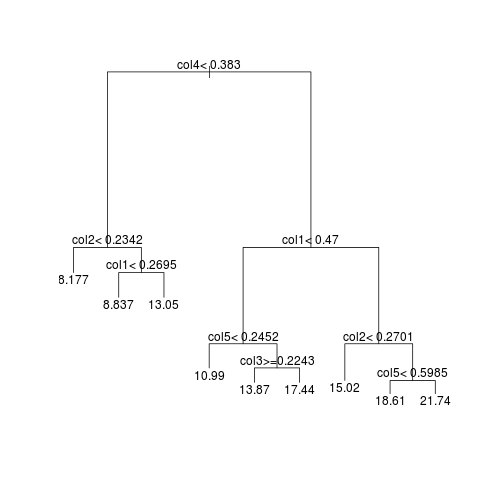
\includegraphics[totalheight=9cm]{./figs/tree_function.png}
 \captionof{figure}{The tree function.}
  \label{figure:tree_function.png}
\end{figure}


\begin{figure}[tbhp]
 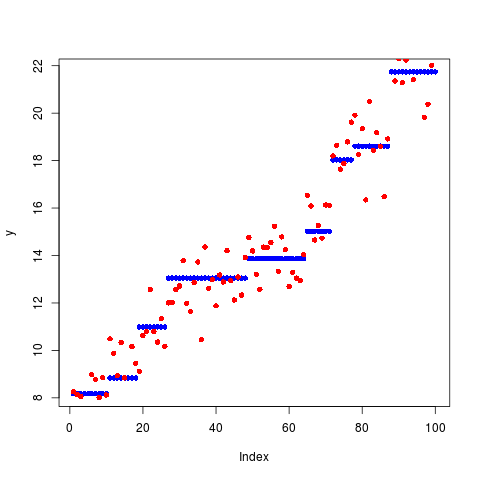
\includegraphics[totalheight=8cm]{./figs/noisy_tree_function.png}
 \captionof{figure}{A plot of the ordered $y$ variable for the tree example, and the $y$ variable with added Gaussian
   noise (in red).}
  \label{figure:noisy_tree_function.png}
\end{figure}










% You may title this section "Methods" or "Models". 
% "Models" is not a valid title for PLoS ONE authors. However, PLoS ONE
% authors may use "Analysis" 
\section*{Methods}




\subsection*{VariantSpark.}



% For figure citations, please use "Fig." instead of "Figure".
%Nulla mi mi, Fig.~\ref{fig1}  Fusce fringilla erat porttitor lectus cursus, \nameref{S1_Video} vel sagittis arcu lobortis. Aliquam in enim semper, aliquam massa id, cursus neque. Praesent faucibus semper libero.
%\begin{figure}[h]
%\caption{{\bf Figure Title first bold sentence Nulla mi mi, venenatis sed ipsum varius, volutpat euismod diam.}
%Figure Caption Proin rutrum vel massa non gravida. Quisque tempor sem et dignissim rutrum. A: Lorem ipsum dolor sit amet. B: Consectetur adipiscing elit.}
%\label{fig1}
%\end{figure}
%\begin{enumerate}
%\item{react}
%\item{diffuse free particles}
%\item{increment time by dt and go to 1}
%\end{enumerate}

% Results and Discussion can be combined.
% Please do not create a heading level below \subsection. For 3rd level headings, use \paragraph{}. 
\section*{Results and Discussion}


%OPTIONS
% Spark ML vs MLlib
% random forest, kmeans, logistic regression 
% synthetic data demonstrating random forest can cope with n<<p
% James dataset
% GWAS dataset


\subsection*{Synthetic data demonstrating that RF can deal with extreme dimensionality}
Detailing random association between features and labels
and whatever rob did


\subsection*{CursedForest copes with the curse of dimensionality}
\label{comp}
Spark ML vs CursedForest vs Kmeans vs LR on small and full version (where applicable) of 1000G (performance and time/mem)

%In this section we compare Apache's higher level machine learning library, Spark ML, with MLLib, the standard low-level library. From the results, we see that times are similar. 
%There are many practical benefits for using Spark ML with VariantSpark, with a selection of these benefits derived from the `pipeline' system Spark ML uses.
%One benefit is that hyperparameter optimisation is built in. Although possible in 



%\subsection*{CursedForest copes with the curse of dimensionality}
%With Spark ML unable to cope with high-dimensional data, we develop a `wide' implementations of these ML algorithms. **technical stuff by Piotr here**
%These 



\subsection*{James' dataset}
Comparing CursedForest with feature selection + linear model (performance and time/mem) 



\subsection*{Conclusion}



%\begin{table}[!ht]
%\begin{adjustwidth}{-2.25in}{0in} % Comment out/remove adjustwidth environment if table fits in text column.
%\caption{
%{\bf Table caption Nulla mi mi, venenatis sed ipsum varius, volutpat euismod diam.}}
%\begin{tabular}{|l|l|l|l|l|l|l|l|}
%\hline
%\multicolumn{4}{|l|}{\bf Heading1} & \multicolumn{4}{|l|}{\bf Heading2}\\ \hline
%$cell1 row1$ & cell2 row 1 & cell3 row 1 & cell4 row 1 & cell5 row 1 & cell6 row 1 & cell7 row 1 & cell8 row 1\\ \hline
%$cell1 row2$ & cell2 row 2 & cell3 row 2 & cell4 row 2 & cell5 row 2 & cell6 row 2 & cell7 row 2 & cell8 row 2\\ \hline
%$cell1 row3$ & cell2 row 3 & cell3 row 3 & cell4 row 3 & cell5 row 3 & cell6 row 3 & cell7 row 3 & cell8 row 3\\ \hline
%\end{tabular}
%\begin{flushleft} Table notes Phasellus venenatis, tortor nec vestibulum mattis, massa tortor interdum felis, nec pellentesque metus tortor nec nisl. Ut ornare mauris tellus, vel dapibus arcu suscipit sed.
%\end{flushleft}
%\label{table1}
%\end{adjustwidth}
%\end{table}


\section*{Supporting Information}

% Include only the SI item label in the subsection heading. Use the \nameref{label} command to cite SI items in the text.
\subsection*{S1 Video}
\label{S1_Video}
{\bf Bold the first sentence.}  Maecenas convallis mauris sit amet sem ultrices gravida. Etiam eget sapien nibh. Sed ac ipsum eget enim egestas ullamcorper nec euismod ligula. Curabitur fringilla pulvinar lectus consectetur pellentesque.

\subsection*{S1 Text}
\label{S1_Text}
{\bf Lorem Ipsum.} Maecenas convallis mauris sit amet sem ultrices gravida. Etiam eget sapien nibh. Sed ac ipsum eget enim egestas ullamcorper nec euismod ligula. Curabitur fringilla pulvinar lectus consectetur pellentesque.

\subsection*{S1 Fig}
\label{S1_Fig}
{\bf Lorem Ipsum.} Maecenas convallis mauris sit amet sem ultrices gravida. Etiam eget sapien nibh. Sed ac ipsum eget enim egestas ullamcorper nec euismod ligula. Curabitur fringilla pulvinar lectus consectetur pellentesque.

\subsection*{S2 Fig}
\label{S2_Fig}
{\bf Lorem Ipsum.} Maecenas convallis mauris sit amet sem ultrices gravida. Etiam eget sapien nibh. Sed ac ipsum eget enim egestas ullamcorper nec euismod ligula. Curabitur fringilla pulvinar lectus consectetur pellentesque.

\subsection*{S1 Table}
\label{S1_Table}
{\bf Lorem Ipsum.} Maecenas convallis mauris sit amet sem ultrices gravida. Etiam eget sapien nibh. Sed ac ipsum eget enim egestas ullamcorper nec euismod ligula. Curabitur fringilla pulvinar lectus consectetur pellentesque.

\section*{Acknowledgments}
Cras egestas velit mauris, eu mollis turpis pellentesque sit amet. Interdum et malesuada fames ac ante ipsum primis in faucibus. Nam id pretium nisi. Sed ac quam id nisi malesuada congue. Sed interdum aliquet augue, at pellentesque quam rhoncus vitae.

\nolinenumbers

%\section*{References}
% Either type in your references using
% \begin{thebibliography}{}
% \bibitem{}
% Text
% \end{thebibliography}
%
% OR
%
% Compile your BiBTeX database using our plos2015.bst
% style file and paste the contents of your .bbl file
% here.
% 

\bibliography{./CursedForest.bib}

\end{document}

